
\documentclass[conference]{IEEEtran}
\IEEEoverridecommandlockouts

% -------------------- PACKAGES --------------------
\usepackage[T1]{fontenc}
\usepackage{cite}
\usepackage{url}
\usepackage{graphicx}
\usepackage{booktabs}
\usepackage{tabularx}
\usepackage{array}
\usepackage{multirow}
\usepackage{enumitem}
\usepackage{tikz}
\usetikzlibrary{arrows.meta,positioning,shapes.geometric,fit,calc}
\usepackage{balance}
\usepackage{microtype}

% -------------------- FORMATTING --------------------
\setlist{nosep,leftmargin=*}
\renewcommand{\arraystretch}{1.12}
\newcolumntype{Y}{>{\raggedright\arraybackslash}X}

% -------------------- TITLE --------------------
\title{Software Requirements Specification for the Electronics Store Inventory Management System (SEIMS)}

% -------------------- AUTHORS --------------------
\author{
\IEEEauthorblockN{Karthik Peddibhotla}
\IEEEauthorblockA{
\textit{Department of Computer Science \& Engineering}\\
PES University\\
SRN: PES2UG24CS348\\
karthikpeddibhotla5@gmail.com}
\and
\IEEEauthorblockN{Paridhi Bajpai}
\IEEEauthorblockA{
\textit{Department of Computer Science \& Engineering}\\
PES University\\
SRN: PES2UG24CS337\\
paridhi.bajaj03@gmail.com}
\and
\IEEEauthorblockN{Niharika S Murthy}
\IEEEauthorblockA{
\textit{Department of Computer Science \& Engineering}\\
PES University\\
SRN: PES2UG24CS316\\
niharika.sm0@gmail.com}
\and
\IEEEauthorblockN{P. Dhanush}
\IEEEauthorblockA{
\textit{Department of Computer Science \& Engineering}\\
PES University\\
SRN: PES2UG24CS333\\
penchalpaadudhanush@gmail.com}
}

\begin{document}

\maketitle

% -------------------- ABSTRACT --------------------
\begin{abstract}
This Software Requirements Specification (SRS) defines the functional, non-functional, interface, data, security, and behavioral requirements for the Electronics Store Inventory Management System (SEIMS), developed for the Software Engineering course (UE24CS302) at PES University. The system is a browser-based application for managing electronic component inventory. It provides user authentication, dashboard summaries, component record management, search and filtering, stock classification, availability reporting, and CSV export.
\end{abstract}

\begin{IEEEkeywords}
Software Requirements Specification, SEIMS, inventory management, Flask, SQLite, requirements engineering, software testing.
\end{IEEEkeywords}

% ==================================================
\section{Introduction}
% ==================================================

\subsection{Purpose}

This document specifies the requirements for the Electronics Store Inventory Management System. It serves as a baseline for system development, architectural design, testing, and project evaluation. It describes what the system is expected to do and the quality and security constraints that apply.

\subsection{Scope}

SEIMS is a web-based application intended to support electronic component inventory tracking and management. Its capabilities include secure user authentication, dashboard summary analytics, component Create, Read, Update, and Delete (CRUD) operations, name-based search, category and availability filtering, stock classification (Available, Low Stock, and Out of Stock), availability reporting, and CSV export.

\subsection{Definitions and Acronyms}

\begin{table}[!t]
\caption{Definitions and Acronyms}
\label{tab:acronyms}
\centering
\small
\begin{tabularx}{\columnwidth}{lY}
\toprule
\textbf{Term} & \textbf{Meaning}\\
\midrule
SRS & Software Requirements Specification\\
SEIMS & Electronics Store Inventory Management System\\
SKU & Stock Keeping Unit\\
CRUD & Create, Read, Update, and Delete operations\\
Low Stock & Quantity less than or equal to the minimum stock threshold\\
Flask & Python micro web framework\\
SQLite & Embedded relational database engine\\
\bottomrule
\end{tabularx}
\end{table}

\subsection{Document Overview}

The remainder of this document describes the product context, user class, operating environment, functional and non-functional requirements, external interfaces, data requirements, system models, acceptance criteria, and requirement traceability.

% ==================================================
\section{Overall Description}
% ==================================================

\subsection{Product Perspective}

SEIMS functions as an independent, browser-based web application. The frontend uses HTML5, CSS3, and Jinja2 templates. It communicates through HTTP requests with a Python Flask server, which interacts with a persistent SQLite database (\texttt{database.db}) and returns rendered HTML pages or CSV data.

\subsection{Product Functions}

The system is intended to:
\begin{itemize}
\item Authenticate store personnel using a username and password.
\item Display dashboard counts for total components, total quantity, low-stock items, and out-of-stock items.
\item Create, view, edit, and delete component records.
\item Search component records by name and filter by category or availability.
\item Classify stock as Available, Low Stock, or Out of Stock.
\item Generate stock availability reports.
\item Export inventory records as downloadable CSV files.
\end{itemize}

\subsection{User Classes}

The principal user class is the Admin/Store Manager. Users are expected to have basic web-navigation skills and familiarity with electronic components such as microcontrollers, sensors, integrated circuits, and passive components.

\subsection{Operating Environment}

\begin{itemize}
\item Server runtime: Python 3.10 or later.
\item Web framework: Flask.
\item Database engine: SQLite 3.
\item Client: A modern browser such as Chrome, Firefox, Safari, or Edge.
\item Local development communication: HTTP over TCP port 5000.
\end{itemize}

\subsection{Design Constraints, Assumptions, and Dependencies}

The system is developed using Python Flask, HTML/CSS, and SQLite. State-changing inventory endpoints require an authenticated session. Database path configuration supports an environment variable with a fallback to \texttt{database.db}. The system assumes that an initial administrative account exists and that client devices can connect to the Flask server.

% ==================================================
\section{Specific Requirements}
% ==================================================

\subsection{Functional Requirements}

Table~\ref{tab:functional} lists the functional requirements. Priority indicates the relative importance of each requirement.

\begin{table*}[!t]
\caption{Functional Requirements Specification}
\label{tab:functional}
\centering
\small
\begin{tabularx}{\textwidth}{l l Y c}
\toprule
\textbf{ID} & \textbf{Name} & \textbf{Description} & \textbf{Priority}\\
\midrule
FR-01 & User Login & Authenticate a user using a username and password. & High\\
FR-02 & User Logout & Clear the active user session when the user logs out. & High\\
FR-03 & Access Control & Restrict unauthenticated access to protected routes. & High\\
FR-04 & Dashboard Summary & Display total, available, low-stock, and out-of-stock counts. & Medium\\
FR-05 & View Inventory & Display component records and their attributes in a table. & High\\
FR-06 & Add Component & Create a component record with name, category, quantity, price, and minimum stock level. & High\\
FR-07 & Edit Component & Modify an existing component record and update the database. & High\\
FR-08 & Delete Component & Delete a selected component using a state-changing request handler. & Medium\\
FR-09 & Search Inventory & Search component records by substring matching on component name. & Medium\\
FR-10 & Category Filter & Filter displayed records by component category. & Medium\\
FR-11 & Status Filter & Filter records by Available, Low Stock, or Out of Stock status. & Medium\\
FR-12 & Clear Filters & Reset search and filter criteria to the default listing. & Low\\
FR-13 & Stock Classification & Calculate stock status using quantity and minimum stock level. & High\\
FR-14 & Availability Report & Generate a grouped report of available, low-stock, and out-of-stock items. & Medium\\
FR-15 & CSV Export & Return inventory data as a downloadable CSV file. & High\\
FR-16 & SKU Uniqueness & Reject insertion or edits that create a duplicate SKU. & High\\
FR-17 & Input Validation & Validate required text fields and non-negative quantities and prices. & High\\
\bottomrule
\end{tabularx}
\end{table*}

\subsection{External Interface Requirements}

\subsubsection{User Interface}

The user interface consists of responsive web templates, including \texttt{login.html}, \texttt{dashboard.html}, \texttt{inventory.html}, \texttt{add\_component.html}, \texttt{edit\_component.html}, and \texttt{report.html}. Styling is provided through the project's CSS stylesheet.

\subsubsection{Software Interfaces}

The backend uses Flask routing and request handlers. Database operations use Python's \texttt{sqlite3} module, including row-based access through \texttt{sqlite3.Row} where configured.

\subsubsection{Communication Interfaces}

The application uses HTTP/1.1 over TCP port 5000 in the local development environment. HTTPS is required for a production deployment.

\subsection{Non-Functional Requirements}

\begin{table*}[!t]
\caption{Non-Functional and Security Requirements}
\label{tab:nfr}
\centering
\small
\begin{tabularx}{\textwidth}{l l Y Y}
\toprule
\textbf{ID} & \textbf{Category} & \textbf{Requirement} & \textbf{Target / Evidence}\\
\midrule
NFR-01 & Usability & Provide understandable forms, stock-status indicators, and feedback messages. & Task completion target: under 30 seconds.\\
NFR-02 & Performance & Provide responsive page loading for the intended inventory workload. & Target: under 2.0 seconds with 1,000 components; measurement required.\\
NFR-03 & Reliability & Preserve committed database records across application restarts. & Verify persistence through restart testing.\\
NFR-04 & Maintainability & Separate templates, styles, and application logic into maintainable units. & Modular project structure.\\
NFR-05 & Portability & Support execution on Windows, Linux, and macOS. & Python 3.10 or later.\\
SEC-01 & Security & Store passwords as cryptographic hashes using the configured Werkzeug password-hashing helper. & No plaintext password storage.\\
SEC-02 & Security & Protect state-changing endpoints using authenticated-session checks. & Unauthenticated edits are denied.\\
SEC-03 & Security & Clear session state when a user logs out. & Session is invalidated.\\
SEC-04 & Security & Use parameterized SQL queries for database operations. & Avoid SQL injection through query parameterization.\\
\bottomrule
\end{tabularx}
\end{table*}

% ==================================================
\section{System Models}
% ==================================================

\subsection{System Context}

Fig.~\ref{fig:context} illustrates the interaction between the Store Manager, browser, Flask backend, and SQLite database.

\begin{figure}[!t]
\centering
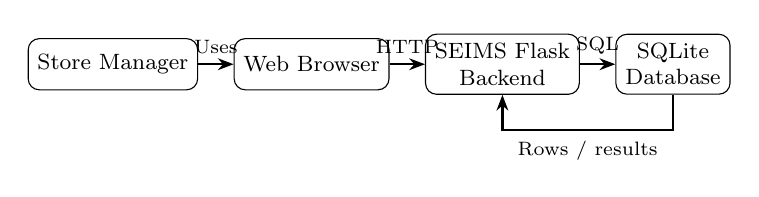
\begin{tikzpicture}[
node distance=0.55cm and 0.45cm,
n/.style={
draw,
rounded corners,
align=center,
minimum width=1.45cm,
minimum height=0.65cm,
font=\footnotesize
},
a/.style={-{Stealth[length=2mm]},thick}
]

\node[n] (user) {Store Manager};
\node[n,right=of user] (browser) {Web Browser};
\node[n,right=of browser] (flask) {SEIMS Flask\\Backend};
\node[n,right=of flask] (db) {SQLite\\Database};

\draw[a] (user)--node[above,font=\scriptsize]{Uses}(browser);
\draw[a] (browser)--node[above,font=\scriptsize]{HTTP}(flask);
\draw[a] (flask)--node[above,font=\scriptsize]{SQL}(db);

\draw[a] (db.south) -- ++(0,-0.45)
-| node[below,pos=0.25,font=\scriptsize]{Rows / results}
(flask.south);

\end{tikzpicture}
\caption{SEIMS System Context}
\label{fig:context}
\end{figure}

\subsection{Use Cases}

The primary actor is the Store Manager. The use cases are:

\begin{itemize}
\item UC-01: User Login
\item UC-02: View Dashboard
\item UC-03: Manage Inventory
\item UC-04: Search and Filter Inventory
\item UC-05: View Stock Availability Report
\item UC-06: Export CSV Data
\item UC-07: User Logout
\end{itemize}

\begin{figure}[!t]
\centering
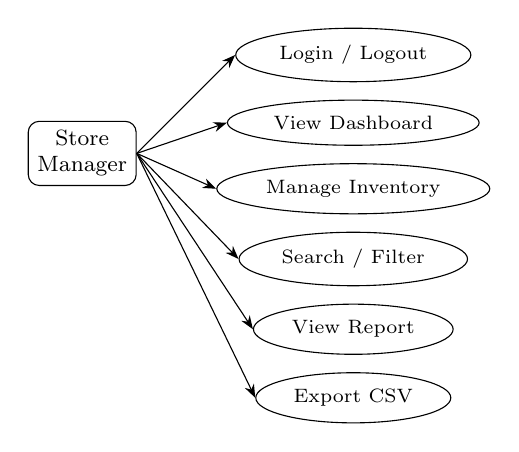
\begin{tikzpicture}[
actor/.style={
draw,
rounded corners,
align=center,
minimum width=1.25cm,
minimum height=0.55cm,
font=\footnotesize
},
use/.style={
draw,
ellipse,
align=center,
minimum width=1.65cm,
minimum height=0.55cm,
font=\scriptsize
},
a/.style={-{Stealth[length=1.7mm]},thin}
]

\node[actor] (manager) {Store\\Manager};

\node[use,right=1.25cm of manager,yshift=1.25cm] (login)
{Login / Logout};

\node[use,below=0.22cm of login] (dash)
{View Dashboard};

\node[use,below=0.22cm of dash] (manage)
{Manage Inventory};

\node[use,below=0.22cm of manage] (filter)
{Search / Filter};

\node[use,below=0.22cm of filter] (report)
{View Report};

\node[use,below=0.22cm of report] (csv)
{Export CSV};

\foreach \x in {login,dash,manage,filter,report,csv}
{
\draw[a] (manager.east)--(\x.west);
}

\end{tikzpicture}
\caption{SEIMS Use-Case Overview}
\label{fig:usecase}
\end{figure}

% ==================================================
\section{Data Requirements}
% ==================================================

\subsection{Data Entities}

The system stores user and component information. The component entity includes \texttt{component\_id} (integer primary key), \texttt{sku} (unique text), \texttt{component\_name}, \texttt{category}, \texttt{quantity} (non-negative integer), \texttt{price} (non-negative real), and \texttt{min\_stock\_level} (non-negative integer, default 10). The user entity includes \texttt{user\_id} (integer primary key), \texttt{username} (unique text), and \texttt{password\_hash}.

\begin{table}[!t]
\caption{Component Table Schema}
\label{tab:schema}
\centering
\small
\begin{tabularx}{\columnwidth}{l l Y}
\toprule
\textbf{Column} & \textbf{Type} & \textbf{Constraint}\\
\midrule
component\_id & INTEGER & Primary key, auto-increment\\
sku & TEXT & Unique, not null\\
component\_name & TEXT & Not null\\
category & TEXT & Not null\\
quantity & INTEGER & Not null, value $\geq 0$\\
price & REAL & Not null, value $\geq 0$\\
min\_stock\_level & INTEGER & Default 10, value $\geq 0$\\
\bottomrule
\end{tabularx}
\end{table}

\begin{table}[!t]
\caption{User Table Schema}
\label{tab:user-schema}
\centering
\small
\begin{tabularx}{\columnwidth}{l l Y}
\toprule
\textbf{Column} & \textbf{Type} & \textbf{Constraint}\\
\midrule
user\_id & INTEGER & Primary key, auto-increment\\
username & TEXT & Unique, not null\\
password\_hash & TEXT & Not null; stores password hash\\
\bottomrule
\end{tabularx}
\end{table}

% ==================================================
\section{Acceptance Criteria}
% ==================================================

The system is considered acceptable when the following criteria are demonstrated:

\begin{enumerate}
\item AC-01 (Security): Unauthenticated users are redirected to the login page when accessing protected routes.
\item AC-02 (CRUD): Creating a component updates the stored inventory records.
\item AC-03 (Classification): Stock status is correctly classified as Out of Stock, Low Stock, or Available according to the implemented threshold logic.
\item AC-04 (Export): The downloaded CSV contains the inventory data returned by the export function.
\item AC-05 (Automated Testing): The automated test suite executes successfully.
\end{enumerate}

% ==================================================
\section{Requirements Traceability}
% ==================================================

\begin{table*}[!t]
\caption{Requirements Traceability Matrix}
\label{tab:rtm}
\centering
\small
\begin{tabularx}{\textwidth}{l l l}
\toprule
\textbf{Requirement IDs} & \textbf{Module} & \textbf{Test File}\\
\midrule
FR-01--FR-03 & Authentication & \texttt{tests/test\_app.py}\\
FR-04 & Dashboard & \texttt{tests/test\_frontend.py}\\
FR-05--FR-08 & Product CRUD & \texttt{tests/test\_inventory\_backend.py}\\
FR-09--FR-12 & Search and Filtering & \texttt{tests/test\_frontend.py}\\
FR-13 & Stock Classifier & \texttt{tests/test\_inventory\_backend.py}\\
FR-14 & Availability Reporting & \texttt{tests/test\_app.py}\\
FR-15 & CSV Export & \texttt{tests/test\_app.py}\\
FR-16--FR-17 & Validation & \texttt{tests/test\_inventory\_backend.py}\\
\bottomrule
\end{tabularx}
\end{table*}

% ==================================================
\section{Appendix: Project Verification Notes}
% ==================================================

The project repository contains the Flask application, HTML templates, CSS assets, and automated Pytest suites. The project team has reported a local test execution result of 39 passing tests and a successful GitHub Actions workflow run. These are reported project results and should be refreshed against the latest repository state before final submission.

% ==================================================
\section{References}
% ==================================================

\begin{thebibliography}{00}

\bibitem{ieee830}
IEEE, \emph{IEEE Recommended Practice for Software Requirements Specifications}, IEEE Std 830-1998, 1998.

\bibitem{python}
Python Software Foundation, ``Python Documentation.''
[Online]. Available: \url{https://docs.python.org/3/}

\bibitem{flask}
Pallets Projects, ``Flask Documentation.''
[Online]. Available: \url{https://flask.palletsprojects.com/}

\bibitem{sqlite}
SQLite Development Team, ``SQLite Documentation.''
[Online]. Available: \url{https://www.sqlite.org/docs.html}

\end{thebibliography}

\balance

\end{document}
